This section presents some experiments on the SC/2R and RPCL models to highlight their similarities and differences. The results are compared to experimental data when available. The code used to generate these results is available at \url{https://github.com/antmaier/Projet-de-Master.git}.

\subsection{Dynamics comparison}
    We begin by simulating some trajectories of the two models under ideal conditions and compute some statistics. In Fig.~\ref{fig:trajectories}, we show some sample trajectories of the two models in solid colored lines, the analytical expected substrate translocation and standard deviation using Eqs.~\eqref{eq:first-moment}~and~\eqref{eq:variance-and-std} in grey solid line and pale colored areas, the empirical standard deviation in dashed lines, and the ATP consumption per translocated residue. We plot as well the distribution of sojourn times between translocation events.

    To compare the two models, their rates are scaled by a factor so that their analytical average velocity is normalized. The constants' exact values are irrelevant; the essential point is that [ATP]/[ADP] concentration ratio is set to a large value similar to in vivo conditions, and its equilibrium value very small, which results in a non-zero average substrate translocation velocity of the AAA+ ATPase. All the other free parameters are set to values of the order of 1 before renormalization.

    \begin{figure}[h]
    \centering
    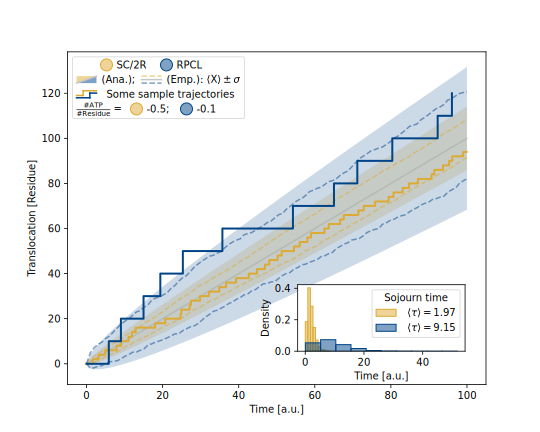
\includegraphics[width=\textwidth]{images/trajectories.pdf}
    \caption{Trajectories and statistical analyses comparing SC/2R (yellow) and RPCL (blue) models of AAA+ ATPase substrate translocation mechanism. Solid colored lines represent sample trajectories for each model, grey solid line and pale areas depict analytical expected substrate translocation and standard deviation, and dashed lines show empirical standard deviation. Empirical ATP consumption per translocated residue and distribution of sojourn times between translocation events are computed. Physical rates are scaled for normalized average velocity, with constants adjusted to maintain ATPase activity.}
    \label{fig:trajectories}
    \end{figure}
    
    As predicted by the calculations in Secs.~\ref{subsec:sc2r-model}~and~\ref{subsec:rpcl-model}, RPCL consumes five times less ATP than SC/2R for a similar average velocity, due to substrate translocation steplength and sojourn time five times longer consuming a single ATP molecule, as visible on the sample trajectories and sojourn times histograms. RPCL dynamics are more consistent with experimental data where it has been shown that the ATPase moves by steps of $14.6\pm 0.9$ amino acids for single-strand translocation\cite{avellaneda_processive_2020}, the setup we simulate in this work.
    
    One behavior that we fail to understand is the discrepancy between analytical and numerical standard deviations. With a convergence analysis, we have ruled out the hypothesis of a sampling error. We suspect that our analytical expression Eq.~\eqref{eq:variance-and-std}) is incorrect, but this issue has not yet been resolved.

\subsection{Adding an external force}
\label{subsec:force}
    Now, we investigate how the dynamics are modified in the presence of an external constant force pulling on the substrate, opposing the AAA+ ATPase translocation. The force thus derives from a potential energy $U(x) \propto x$, where $x$ is the substrate translocated length, and we fix $u$ the potential energy for a unit translocation $\Delta x = 1$ residue. Following the Arrhenius law, the presence of this potential modifies the rate of reactions that induce a substrate translocation $\Delta x$ by $k\mapsto k e^{-\beta u \Delta x }$, where $\beta$ is the inverse temperature, and we assume that the pre-exponential factor is already contained in the rate $k$. This additional Boltzmann factor does not influence the thermodynamic loop law Eq.~\eqref{eq:thermo-loop-law} since at equilibrium, the force is zero, the potential energy is constant, and thus for any reaction that induces a substrate translocation $\Delta x$, the Boltzmann factor equals one. Therefore, a rate constrained by the loop law is similarly modified, i.e. $k\mapsto k e^{-\beta u \Delta x }$, where $k$ is the constrained rate. However, the additional term does influence the dynamics for non-zero forces. Physical quantities are computed by replacing old rates with new ones containing the Boltzmann factor.

    In practical terms, both SC/2R and RPCL models are made of a single loop with a single reaction associated with a translocation of the substrate. Thus, after fixing an arbitrary value $u/T$, the rates are transformed as follows:
    \begin{itemize}
        \item $k_\uparrow\mapsto k_\uparrow e^{-2 \frac{u}{T}}$ and $k_\downarrow\mapsto k_\downarrow e^{2 \frac{u}{T}}$ for SC/2R;
        \item $k_{\uparrow ext.} \mapsto k_{\uparrow ext.} e^{-10 \frac{u}{T}}$ and $k_{\downarrow cont.} \mapsto k_{\downarrow cont.} e^{10 \frac{u}{T}}$ for RPCL.
    \end{itemize}
    
    In Fig.~\ref{fig:force}, we show the average velocity as a function of the thermally scaled unit potential energy $u/T$ for both models. It is irrelevant to compare their numerical values here since their rates are set arbitrarily and do not necessarily correspond to the same physical quantities. The key point is the qualitative behavior of the average velocity as a function of the force, which we can see is similar for both models. In particular, we see that the average velocity is modified as soon as we apply a non-zero force. This is an argument in disfavor of the experimental result where the velocity is unaffected by the force up to a threshold value, after which the velocity drastically falls\cite{avellaneda_processive_2020}. However, this result must be taken cautiously due to their high measurement uncertainties.

    \begin{figure}[h]
        \centering
        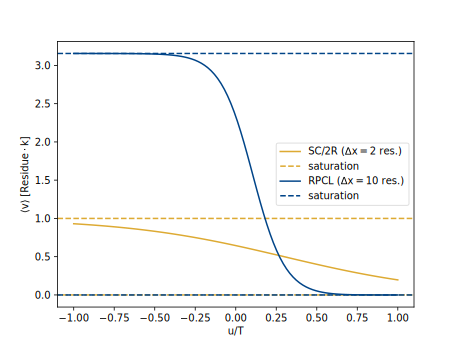
\includegraphics[width=\textwidth]{images/force.pdf}
        \caption{Average substrate translocation velocity as a function of the potential energy for a unit residue translocation over temperature for SC/2R (yellow) and RPCL (blue) models. The potential is generated by a constant force opposing the AAA+ ATPase substrate translocation.}
        \label{fig:force}
    \end{figure}
    
    The second important feature visible in Fig.~\ref{fig:force} is the sigmoidal shape of the average velocity, inversely related to the force. The inverse relation comes from the fact that the force acts as a barrier that the ATPase has to overcome to translocate the substrate and similarly facilitates its translocation in the reverse direction. The saturation comes from the fact that for extreme forces, the reactions associated with a translocation favored by the force in the kinetic scheme have an exponentially big rate so that when the system is in the initial state of the reaction, it will almost instantaneously jump to the resulting state, and similarly, the rate of reactions disfavored by the force is exponentially small so that this reaction is practically never realized. Therefore, the probability flux in the loop in essentially determined by the other reactions.
    
    This result was predictable when looking at the analytical expression of the steady-state probabilities and the average velocity. We illustrate this with the SC/2R model, but it would be similar for RPCL since both models are made of a single loop. Consider a large force intensity that will inhibit the forward translocation of the substrate. Mathematically, this corresponds to the situation $u \rightarrow \infty$, and thus the rates $k_\uparrow \rightarrow 0$ and $k_\downarrow \rightarrow\infty$ while all the other rates are left unchanged. In this limit, the steady-state probabilities Eq.~\eqref{eq:sc2r-steady-state-probabilities} become:
    \begin{equation}
    \begin{split}
        p_A &\propto k_s k_{DT} + k_\downarrow k_s + k_\uparrow k_{DT} 
            \approx k_\downarrow k_s \\
        p_B &\propto k_h k_\downarrow + k_{DT} k_h + k_{TD} k_\downarrow 
            \approx k_\downarrow (k_h + k_{TD}) \\
        p_C &\propto k_\uparrow k_{TD} + k_s k_{TD} + k_h k_\uparrow
            \approx 0
    \end{split}
    \end{equation}
    since $k_\downarrow$ appears in the denominator but not in the numerator of $p_C$, shrinking it to zero. In this limit, $k_\downarrow$ factorizes in $p_A$ and $p_B$, and thus are canceled out by the normalization constant. Therefore, the probabilities are:
    \begin{equation}
    \begin{split}
        p_A &\propto \frac{k_s}{k_s + k_h + k_{TD}} \\
        p_B &\propto \frac{k_h + k_{TD}}{k_s + k_h + k_{TD}}
    \end{split}
    \end{equation}
    The interpretation is that in this limit, the upward protomer translocation $k_\uparrow$ and state $C$ are removed from the kinetic scheme, and a reaction $A\to B$, an $\text{ATP}\to\text{ADP}$ exchange followed immediately by a downward protomer translocation (with rate canceled out), with an effective rate $k_{TD}$ is added. Then state $A$ can only be reached from state $B$ with rate $k_s$, and state $B$ can be reached from $A$ either by hydrolysis with rate $k_h$ or by the newly added effective reaction with rate $k_{TD}$. Consequently, the average velocity Eq.~\eqref{eq:sc2r-average-velocity} becomes:
    \begin{equation}
        \left\langle v \right\rangle \propto - \Delta x k_s k_{TD}
    \end{equation}
    We see in particular that even though in Fig.~\ref{fig:force} the average velocity seems to fall to zero for large forces, it actually saturates to a non-null but negative value. The speed is close to zero since the value of $k_{DT} \sim 1$, [ATP]/[ADP] $\gg 1$ and then $k_{TD}$ being fixed by Eq.~\eqref{eq:kdt-ktd-ratio} results in a very small value.
    
    The same reasoning can also be applied to the other limit $u\rightarrow -\infty$ and to the RPCL model. For the sake of completeness, all the saturated velocities are summarized here:
    \begin{equation}
    \begin{split}
        \left\langle v \right\rangle_{SC/2R} &=
            \begin{cases}
                \Delta x \frac{k_h k_{DT}}{k_h + k_{DT} + k_{TD}},
                    & \text{for } u\rightarrow -\infty \\
                - \Delta x \frac{k_s k_{TD}}{k_s + k_h + k_{TD}},
                    & \text{for } u\rightarrow \infty
            \end{cases} \\
        \left\langle v \right\rangle_{RPCL} &= 
            \begin{cases}
                \Delta x \frac{\bar{k}_h k_{DT} k_{\uparrow cont.}}{k_{DT} k_{\uparrow cont.} + k_{TD} \bar{k}_{\downarrow ext.} + \bar{k}_h k_{TD} + \bar{k}_h k_{\uparrow cont.} + k_{DT} \bar{k}_{\downarrow ext.} + \bar{k}_h k_{DT}}, 
                    & \text{for } u\rightarrow -\infty \\
                - \Delta x \frac{k_s k_{TD} \bar{k}_{\downarrow ext.}}{k_s k_{\uparrow cont.} + k_s k_{TD} + \bar{k}_h k_{TD} + \bar{k}_h k_{\uparrow cont.} + k_{TD} \bar{k}_{\downarrow ext.} + k_s \bar{k}_{\downarrow ext.}},
                    & \text{for } u\rightarrow \infty
            \end{cases}
    \end{split}
    \end{equation}
    and these analytical expressions are represented in dashed lines in Fig~\ref{fig:force}, which shows that the derivation above is consistent with the numerical implementation.
    
    We remember that in the RPCL model, we arbitrarily considered a substrate translocation during the upward extension ($k_{\uparrow ext.}$) and downward contraction ($k_{\downarrow cont.}$) of the ATPase and not during the upward contraction ($k_{\uparrow cont.}$) and downward extension ($k_{\downarrow ext.}$). One could choose instead to consider the translocation during the latter two reactions, or even split it, half the translocation during the former two reactions and half during the latter two reactions. This would not change the qualitative results highlighted here.

\subsection{Defective protomer}
    The last experiment we conduct studies how AAA+ ATPase dynamics are affected when a protomer is defective and hydrolyzes at a reduced rate. All the other characteristics of the defective protomers, in particular the spontaneous synthesis rate, stay unchanged, as well as all the other defectless protomers. 

    The undistinguishability assumption we made when introducing the models no longer holds. For the RPCL model, we consider two loops linked at the fully-ATP-bound-flat configuration, with one loop representing the reaction sequence of the defective protomer and the second loop being the reaction sequence of any $N-1$ defectless protomer, merged into a single loop, similarly as we did in the original model, since in this particular state, any protomer can randomly hydrolyze its ATP molecule. For the SC/2R model, we have no choice but to implement a large loop with the reaction sequence of each protomer consecutively. The defective protomer has a reduced hydrolysis rate $k_h\mapsto \alpha k_h$, where $\alpha$ is the defect factor.

    We show in Fig.~\ref{fig:defective} the effect of this defective protomer on the two models SC/2R and RPCL. With a defect factor $\alpha = 0.1$, SC/2R's average velocity is visibly reduced, both empirically and analytically, in a consistent manner. Compared to the defectless case, we see that the time between translocation events is more irregular, with longer plateaux, which is supported by the heavier-tail on the sojourn times histogram. This is because in this model, when the defective protomer is in the lowest position, there is no other path for the cycle to continue than to wait for it to hydrolyze its ATP molecule, and due to the defect factor, this waiting time is longer. On the other hand, with RPCL, the presence of a defective protomer affects substantially less the average velocity, as we can see on the trajectory and the sojourn times histogram. This is explained by the fact that in this model, the dynamics never depend on the defective protomer to hydrolyze its ATP molecule to continue because all protomers compete in parallel to hydrolyze their ATP molecule, and the only effect is that the defective protomer is less likely to be the first one to do so. Even in the limit $\alpha\rightarrow 0$, it would stay almost unaffected by the defect, whereas, in the SC/2R model, the ATPase would stop entirely. This result is consistent with experimental data where it has been shown that the ATPase is not significantly affected when the hydrolysis rate of a protomer is diminished\cite{desantis_operational_2012}.

    \begin{figure}[h]
        \hspace*{-0.25\textwidth}
        \centering
        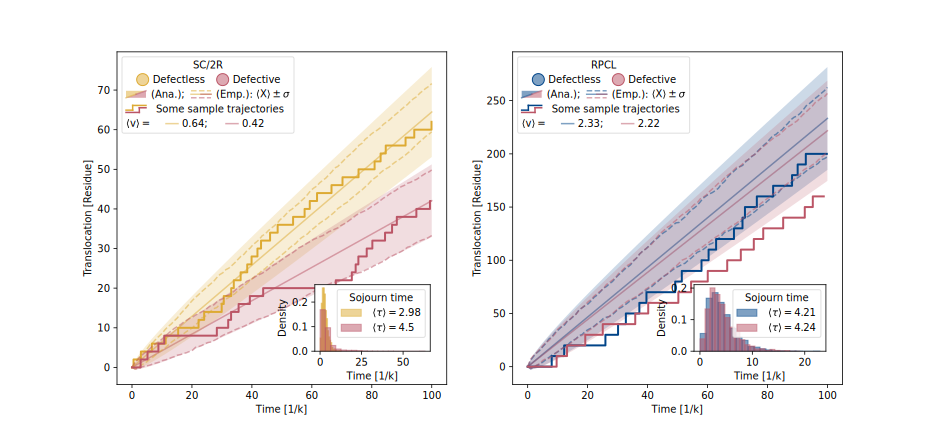
\includegraphics[width=1.5\textwidth]{images/defective.pdf}
        \caption{Comparison of the effects of a defective (red) protomer with hydrolysis rate ten times smaller on the dynamics of SC/2R (yellow) and RPCL (blue) models. Colored solid lines are trajectories, grey solid line and pale areas are analytical expected substrate translocation and standard deviation, dashed lines are empirical standard deviation. Average velocity in defectless and defective cases and the distribution of sojourn times between translocation events are computed. Physical rates are chosen to maintain ATPase activity.}
        \label{fig:defective}
    \end{figure}
